\begin{figure}
	\centering
	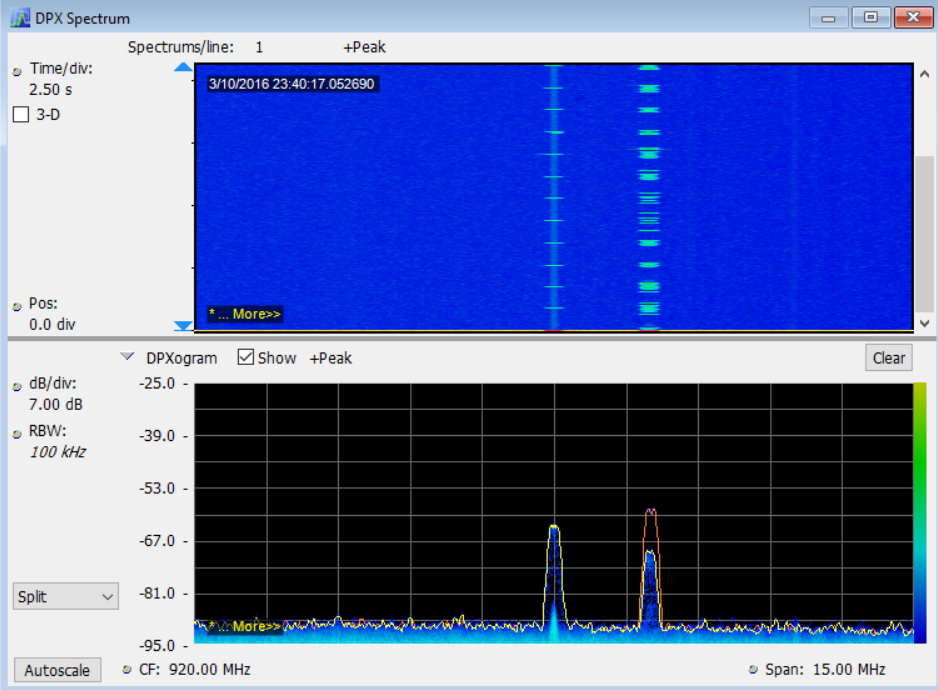
\includegraphics[scale=0.4]{FrequencyShift922-920}
	\caption{The result of using ALFRED to shift frequencies. One node is left behind as the others move to the new channel. Image collected using the Tektronix RSA306 Spectrum Analyzer}
	\label{fig:freqshift}
\end{figure}

\section{Limitations and Future Work}

The results from our experiments show that the network is functioning as a multi hop SDRN. In addition to the experiments performed, we were also able to use Secure Shell (SSH) and Secure Copy (SCP) over multiple hops of the SDRN. However, it is clear that more work needs to be done. In a deployed network, packet loss as high as is seen in this network is not optimal. Therefore, it is important to examine ways to mitigate packet loss and increase throughput. For example, machine learning or artificial intelligence algorithms could be used to adjust transmission parameters as issues are detected. It is likely that a change in frequency or amplitude could mitigate some of the packet loss. For example, if the loss is due to crowding near one node, frequency hopping could be employed to shift to better operating conditions. Batctl's link quality metric, as shown in Figures \ref{fig:2Hops} and \ref{fig:NewHop} could help with finding weak nodes and making decisions. This would be the beginning of ARCAM-Net's transition from a SDRN to a Cognitive Radio Network (CRN). 

Furthermore, it would be beneficial to either improve upon A.L.F.R.E.D. or implement certain features in a new way in order to handle the frequency changing. If we have each node wait for an acknowledgment from its immediate neighbors before changing frequency, that node could then change its frequency knowing that the data will propagate to the rest of the network. Batctl is able to report the immediate next hop neighbors, so the program could use this information to only wait for acknowledgment from neighbors instead of waiting for the entire network to be ready to change. In order for the current A.L.F.R.E.D. setup to function, a delay was needed to give the network time to respond. Therefore, an asynchronous acknowledge would likely speed up the frequency change. 

